\documentclass[12pt,a4paper]{article}
\usepackage[utf8]{inputenc}
\usepackage[margin=0.75in]{geometry}
\usepackage{graphicx}
\usepackage{amsmath}
\usepackage{amssymb}
\usepackage{hyperref}
\usepackage{xcolor}
\usepackage{listings}
\usepackage{float}
\usepackage{booktabs}
\usepackage{array}
\usepackage{caption}
\usepackage{subcaption}
\usepackage{fancyhdr}
\usepackage{setspace}

\lstset{
    basicstyle=\ttfamily\small,
    breaklines=true,
    keywordstyle=\color{blue},
    commentstyle=\color{gray},
    stringstyle=\color{red},
    showstringspaces=false,
    frame=single,
}

\pagestyle{fancy}
\fancyhf{}
\rhead{\thepage}
\lhead{CSL 7640: NLU Assignment 2}

\title{%
    \textbf{CSL 7640: Natural Language Understanding - Assignment 2}\\
    \vspace{0.3cm}
    \large{Word Embeddings and RNN-based Name Generation}
}
\author{Anand Mishra}
\date{March 25, 2026}

\begin{document}

\maketitle
\newpage
\tableofcontents
\newpage

\section{Problem 1: Word Embeddings from IIT Jodhpur Data}

\subsection{Dataset Preparation}

\subsubsection{Collection and Preprocessing}

Data sources: IIT Jodhpur official website, academic regulations, faculty profiles, course syllabi.

Preprocessing pipeline:
\begin{itemize}
    \item Boilerplate and HTML artifact removal
    \item Tokenization and lowercasing
    \item Punctuation normalization
    \item English-only filtering
\end{itemize}

\subsubsection{Dataset Statistics}

\begin{table}[H]
\centering
\begin{tabular}{|l|r|}
\hline
\textbf{Metric} & \textbf{Value} \\
\hline
Documents & 200 \\
Total Tokens & 71,544 \\
Vocabulary Size & 6,628 \\
\hline
\end{tabular}
\caption{Dataset Statistics}
\end{table}

\begin{figure}[H]
    \centering
    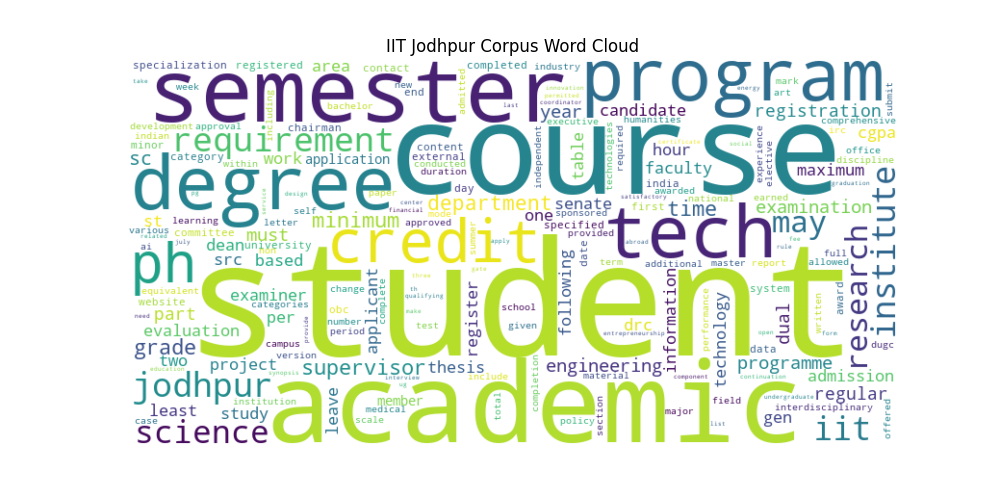
\includegraphics[width=1.0\textwidth]{images/wordcloud.png}
    \caption{Word Cloud - Most Frequent Terms}
\end{figure}

Dominant terms (students, program, course, degree, research) appropriate for academic documents.

\subsection{Model Training and Hyperparameter Experiments}

\subsubsection{Architecture Overview}

\textbf{Skip-gram:} Predicts context words from target word. Effective for semantic relationships and rare words.

\textbf{CBOW:} Predicts target word from context. Computationally efficient, captures co-occurrence patterns.

Both use negative sampling. Experiments: embedding dimension (50, 100, 150), context window (2, 4, 6), negative samples (3, 5, 10).

\subsubsection{Embedding Dimension Impact}

\begin{figure}[H]
    \centering
    \begin{subfigure}{0.32\textwidth}
        \centering
        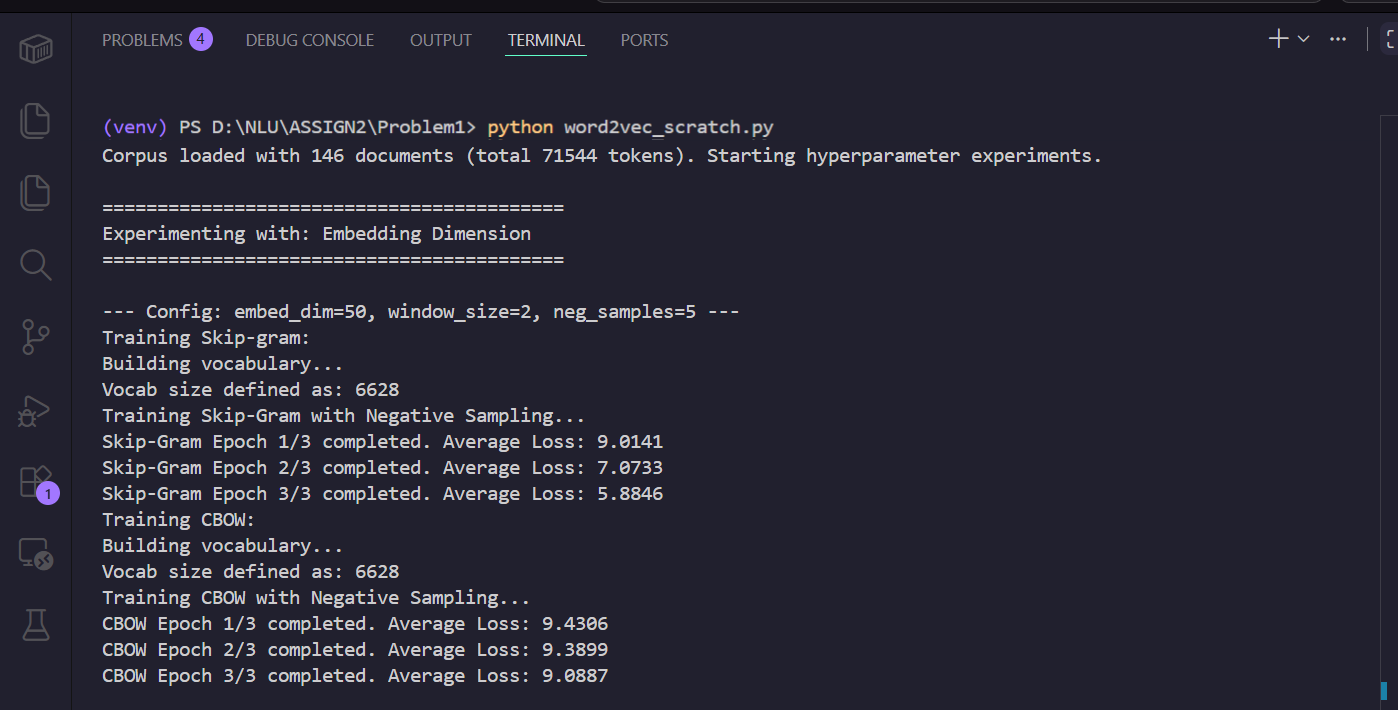
\includegraphics[width=\textwidth]{images/embed_dim_50_que1.png}
        \caption{Dim=50}
    \end{subfigure}
    \begin{subfigure}{0.32\textwidth}
        \centering
        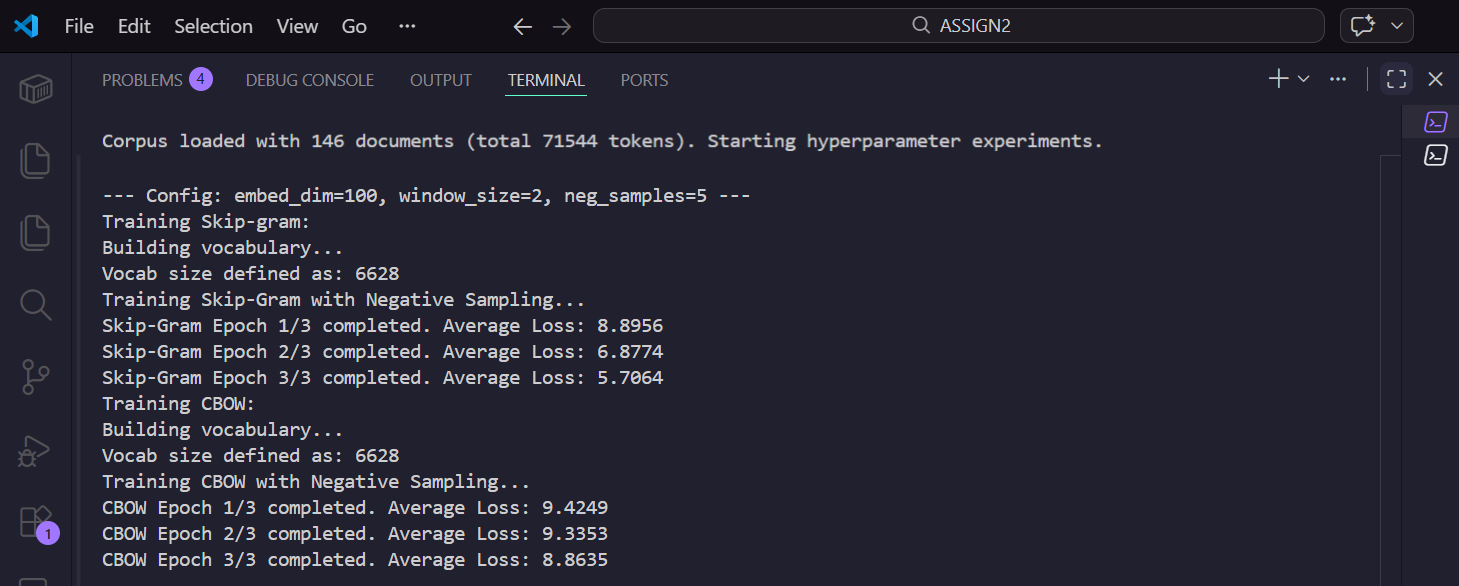
\includegraphics[width=\textwidth]{images/embed_dim_100_que1.png}
        \caption{Dim=100}
    \end{subfigure}
    \begin{subfigure}{0.32\textwidth}
        \centering
        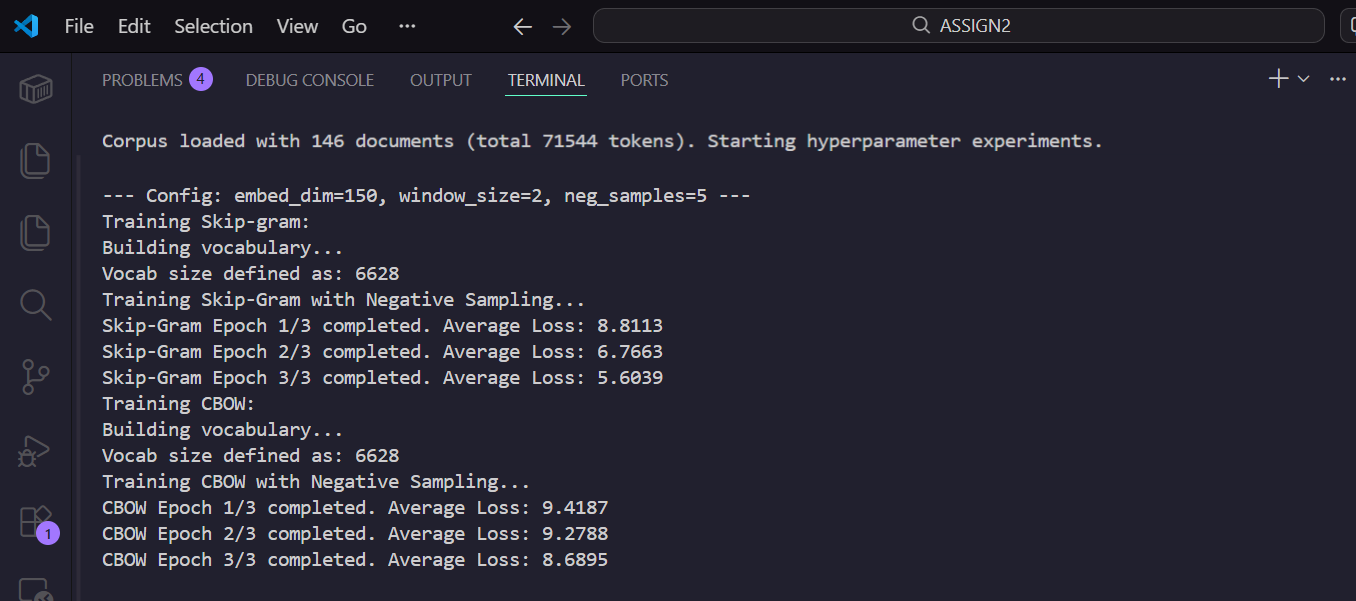
\includegraphics[width=\textwidth]{images/embed_dim_150_que1.png}
        \caption{Dim=150}
    \end{subfigure}
    \caption{Embedding Dimension: Skip-gram Loss 5.88→5.70→5.60 | CBOW Loss 9.09→8.86→8.69}
\end{figure}

Skip-gram improves with larger dimensions; CBOW remains stable. Diminishing returns beyond 100.

\subsubsection{Context Window Size Impact}

\begin{figure}[H]
    \centering
    \begin{subfigure}{0.32\textwidth}
        \centering
        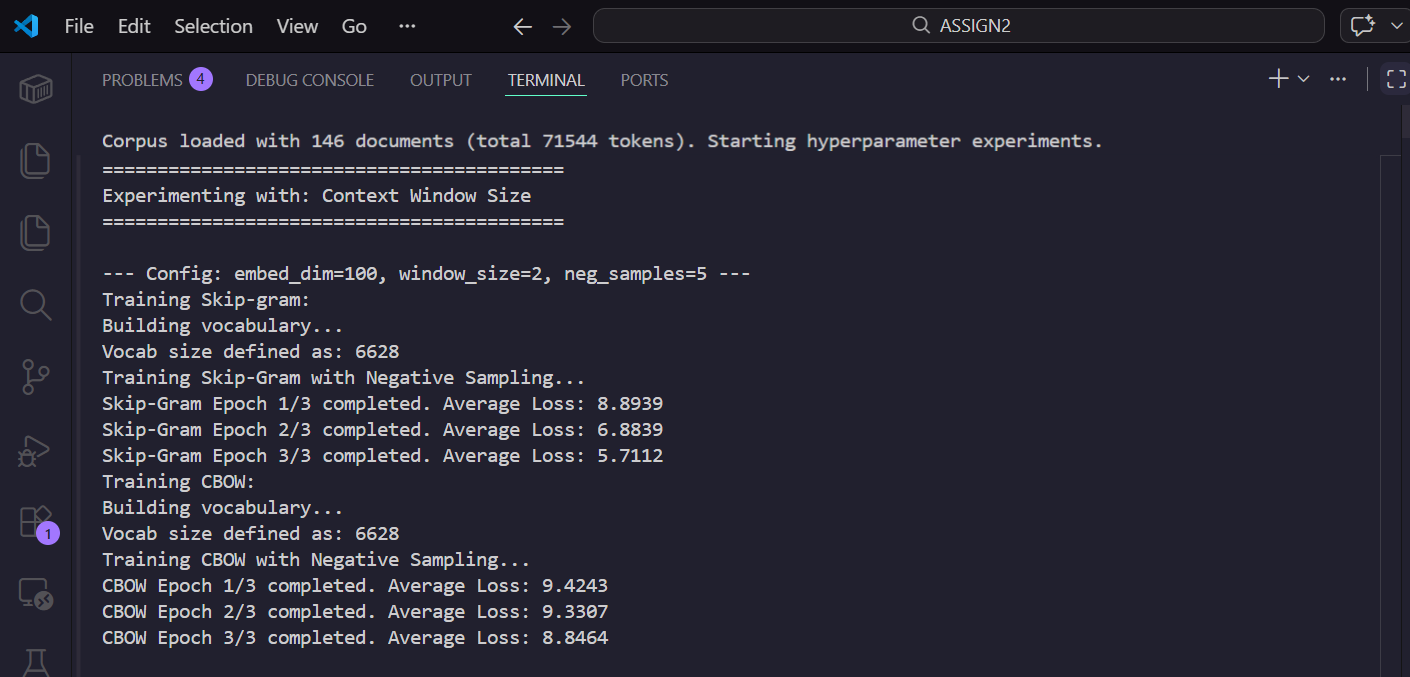
\includegraphics[width=\textwidth]{images/window_size_2_que1.png}
        \caption{Window=2}
    \end{subfigure}
    \begin{subfigure}{0.32\textwidth}
        \centering
        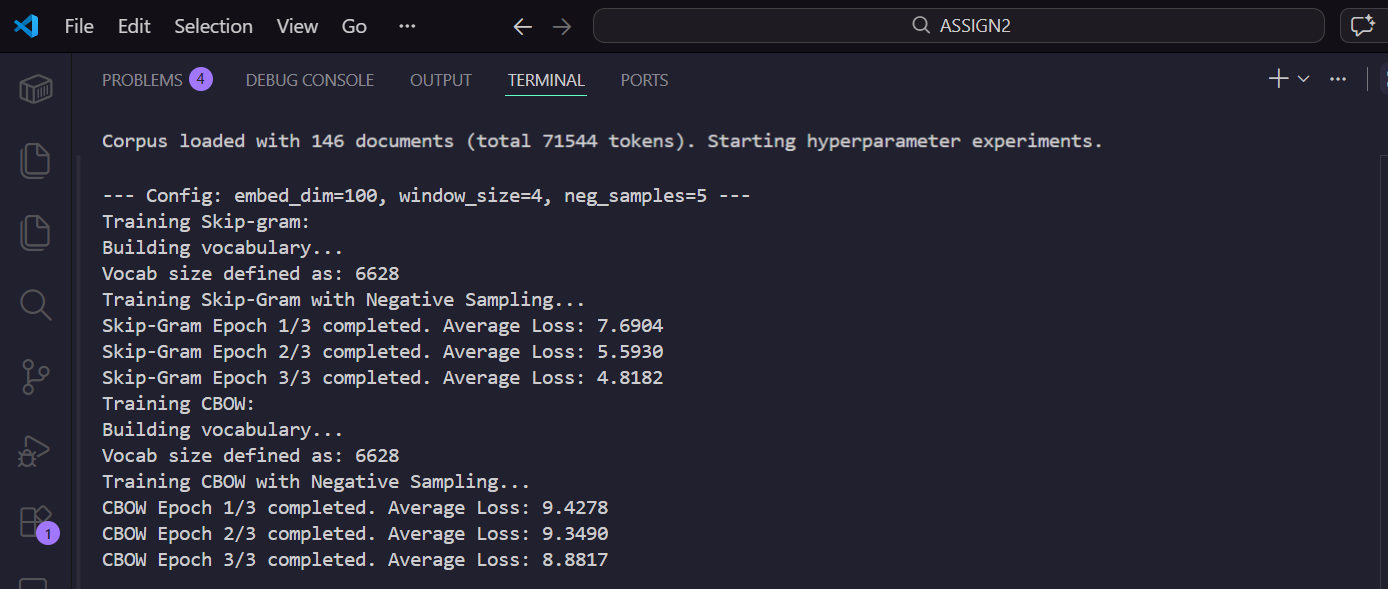
\includegraphics[width=\textwidth]{images/window_size_4_que1.png}
        \caption{Window=4}
    \end{subfigure}
    \begin{subfigure}{0.32\textwidth}
        \centering
        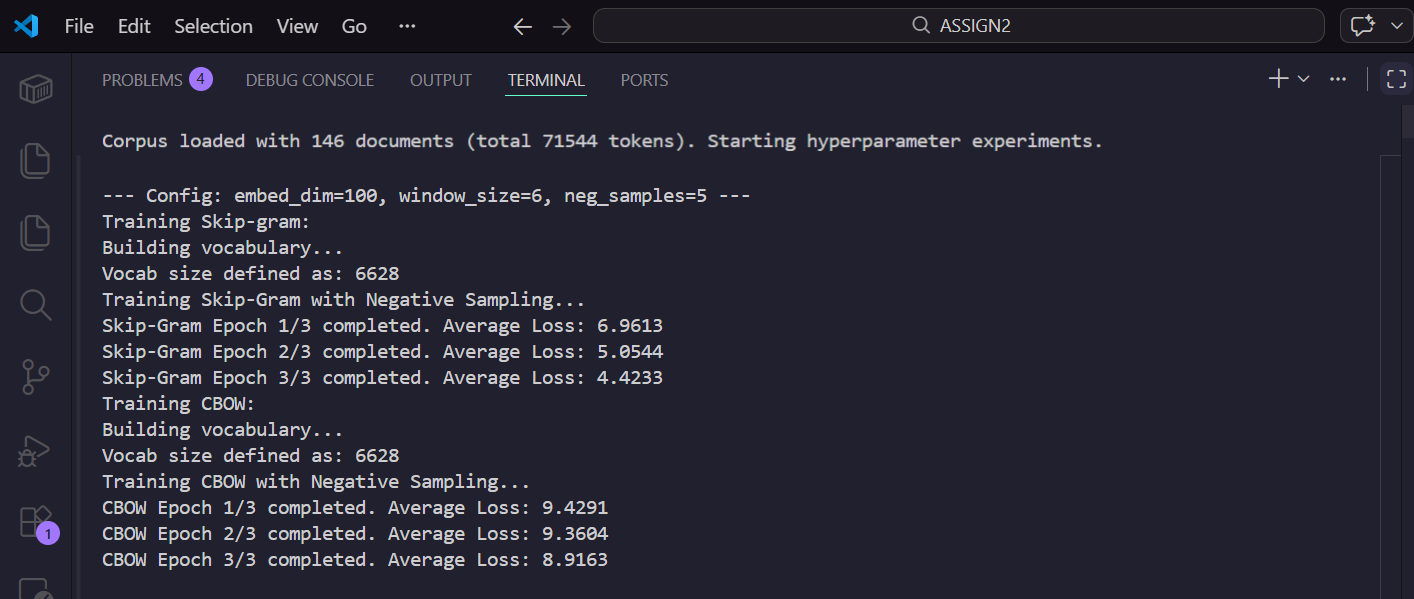
\includegraphics[width=\textwidth]{images/window_size_6_que1.png}
        \caption{Window=6}
    \end{subfigure}
    \caption{Window Size: Skip-gram Loss 5.71→4.82→4.42 | CBOW Loss stable ~8.84-8.91}
\end{figure}

Larger windows significantly improve Skip-gram by capturing distant word relationships. CBOW insensitive to window size.

\subsubsection{Negative Samples Impact}

\begin{figure}[H]
    \centering
    \begin{subfigure}{0.32\textwidth}
        \centering
        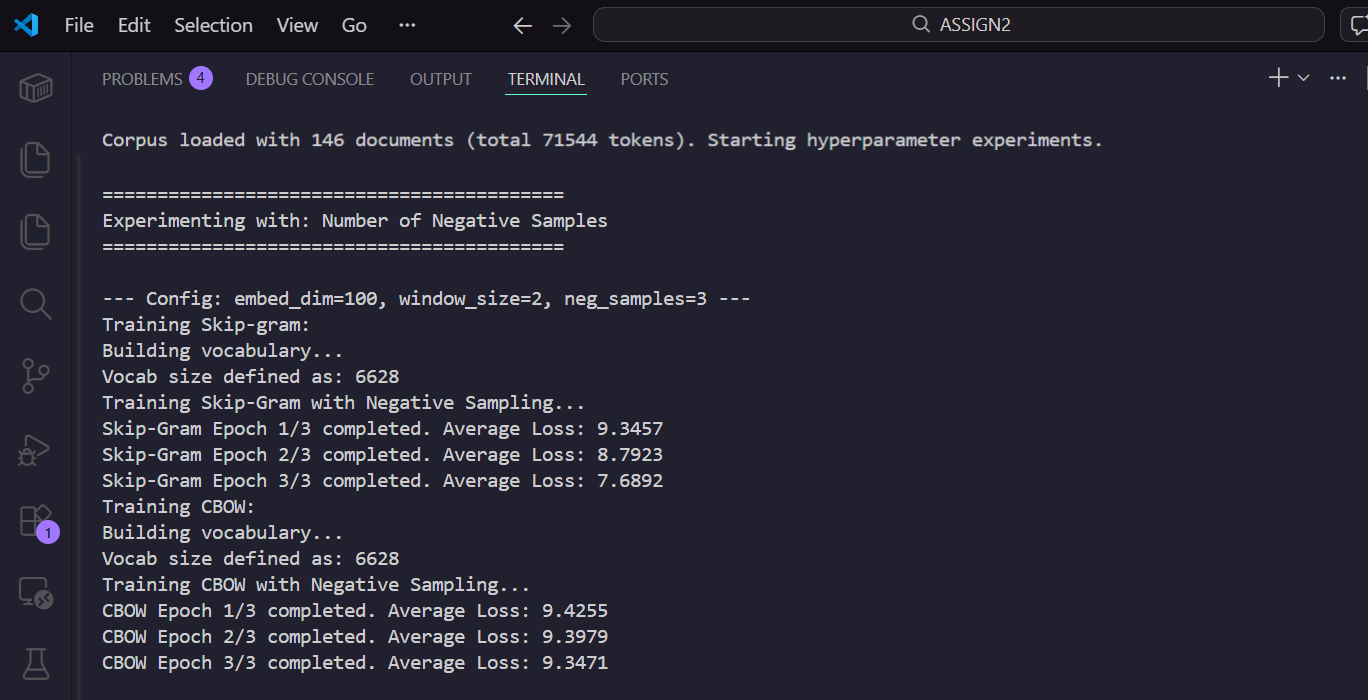
\includegraphics[width=\textwidth]{images/neg_samples_3_que1.png}
        \caption{Neg=3}
    \end{subfigure}
    \begin{subfigure}{0.32\textwidth}
        \centering
        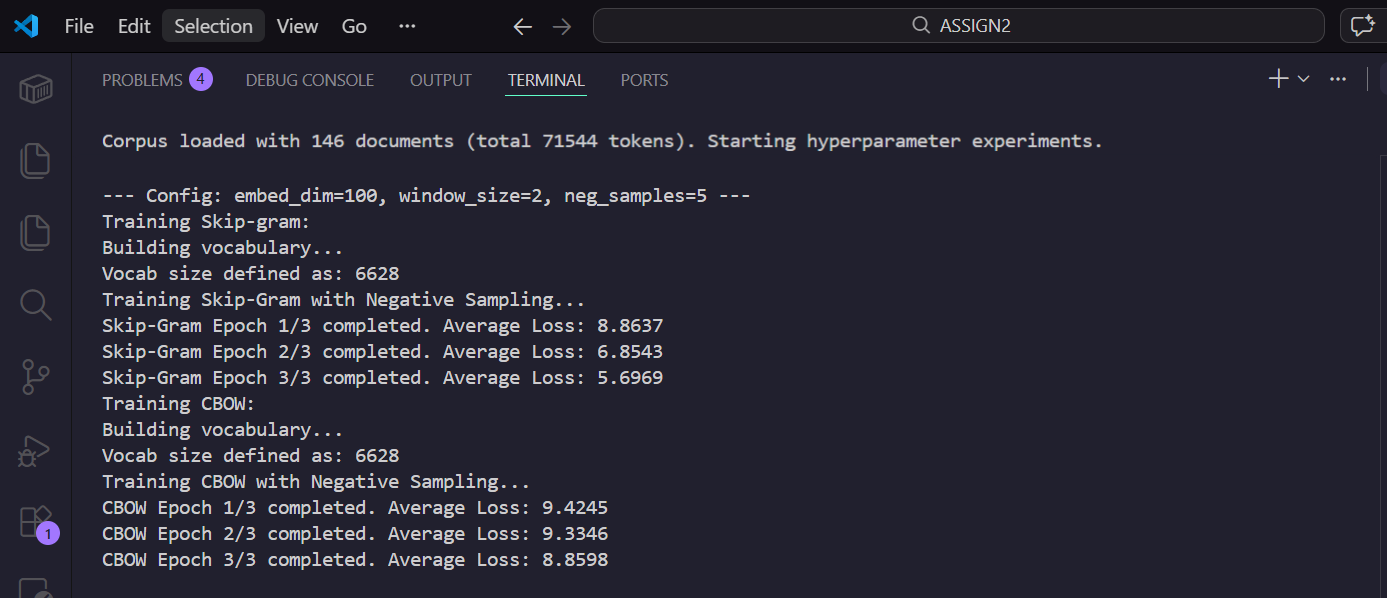
\includegraphics[width=\textwidth]{images/neg_samples_5_que1.png}
        \caption{Neg=5}
    \end{subfigure}
    \begin{subfigure}{0.32\textwidth}
        \centering
        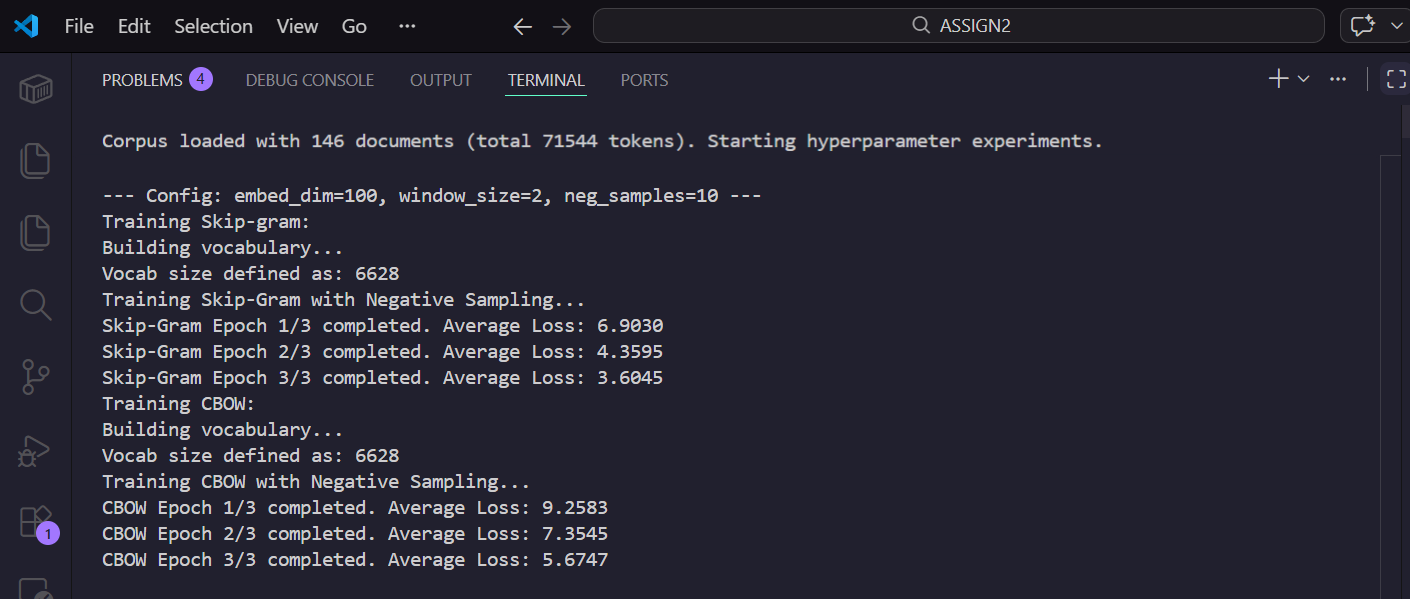
\includegraphics[width=\textwidth]{images/neg_samples_10_que1.png}
        \caption{Neg=10}
    \end{subfigure}
    \caption{Negative Samples: Skip-gram Loss 7.69→5.70→3.60 | CBOW Loss 9.35→8.86→5.67}
\end{figure}

Both models improve substantially with more negative samples. Diminishing returns beyond 10.

\begin{table}[H]
\centering
\small
\begin{tabular}{|c|c|c|c|c|}
\hline
\textbf{Dim} & \textbf{Win} & \textbf{Neg} & \textbf{SG Loss} & \textbf{CBOW Loss} \\
\hline
50 & 2 & 5 & 5.8846 & 9.0887 \\
100 & 2 & 5 & 5.7064 & 8.8635 \\
150 & 2 & 5 & 5.6039 & 8.6895 \\
100 & 2 & 5 & 5.7112 & 8.8464 \\
100 & 4 & 5 & 4.8182 & 8.8817 \\
100 & 6 & 5 & 4.4233 & 8.9163 \\
100 & 2 & 3 & 7.6892 & 9.3471 \\
100 & 2 & 5 & 5.6969 & 8.8598 \\
100 & 2 & 10 & 3.6045 & 5.6747 \\
\hline
\end{tabular}
\caption{Hyperparameter Experiment Results}
\end{table}

\subsection{Semantic Analysis}

\subsubsection{Nearest Neighbors Analysis}

\begin{table}[H]
\centering
\small
\begin{tabular}{|l|c|l|c|}
\hline
\multicolumn{2}{|c|}{\textbf{Skip-gram}} & \multicolumn{2}{|c|}{\textbf{CBOW}} \\
\hline
\textbf{Research Neighbors} & \textbf{Sim} & \textbf{Neighbors} & \textbf{Sim} \\
conversant & 0.762 & students & 0.957 \\
proposal & 0.748 & student & 0.950 \\
work & 0.740 & course & 0.931 \\
\hline
\textbf{Student Neighbors} & \textbf{Sim} & \textbf{Neighbors} & \textbf{Sim} \\
candidate & 0.718 & students & 0.978 \\
semester & 0.726 & program & 0.957 \\
\hline
\textbf{PhD Neighbors} & \textbf{Sim} & \textbf{Neighbors} & \textbf{Sim} \\
dual & 0.942 & tech & 0.652 \\
mtech & 0.938 & degree & 0.624 \\
\hline
\textbf{Exam Neighbors} & \textbf{Sim} & \textbf{Neighbors} & \textbf{Sim} \\
day & 0.906 & certificates & 0.498 \\
mission & 0.907 & maintained & 0.462 \\
\hline
\end{tabular}
\caption{Top Neighbors (Cosine Similarity)}
\end{table}

\textbf{Skip-gram:} Better semantic coherence. Identifies contextually relevant terms (research→proposal, phd→mtech).

\textbf{CBOW:} Strong co-occurrence patterns but less semantic precision. Plural/singular associations dominant.

\begin{figure}[H]
    \centering
    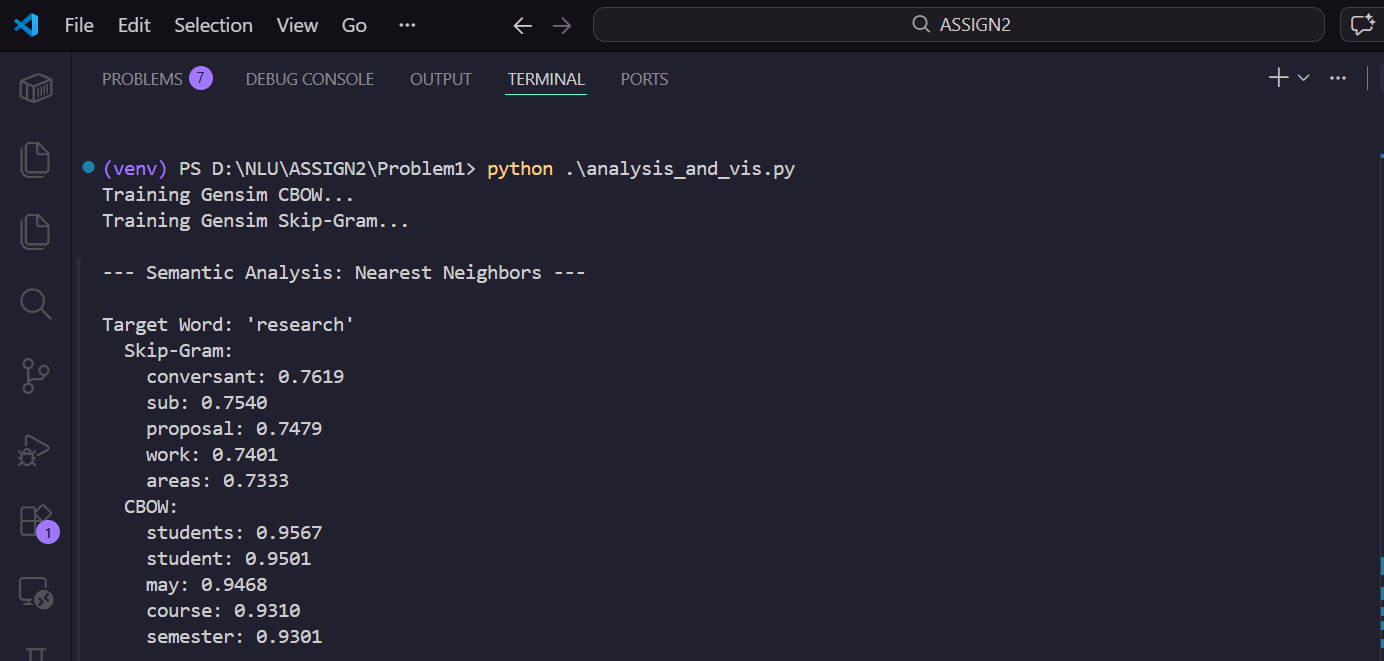
\includegraphics[width=1.0\textwidth]{images/top5Words_example1_que1.png}
    \caption{Nearest Neighbors Example}
\end{figure}

\subsubsection{Analogy Results}

\begin{table}[H]
\centering
\small
\begin{tabular}{|l|c|l|c|}
\hline
\multicolumn{2}{|c|}{\textbf{UG : BTech :: PG : ?}} & \multicolumn{2}{|c|}{\textbf{Faculty : Teaching :: Student : ?}} \\
\hline
Skip-gram: master (0.58) & CBOW: dynamic (0.45) & Skip-gram: semesters (0.65) & CBOW: students (0.96) \\
\hline
\multicolumn{4}{|c|}{\textbf{Research : PhD :: Course : ?}} \\
\hline
\multicolumn{2}{|c|}{Skip-gram: courses (0.73), independent (0.72)} & \multicolumn{2}{|c|}{CBOW: courses (0.79), student (0.81)} \\
\hline
\end{tabular}
\caption{Analogy Experiments}
\end{table}

Best result: Research-PhD-Course analogy where both models identify "courses" correctly. Other analogies weak, indicating insufficient pattern exposure.

\begin{figure}[H]
    \centering
    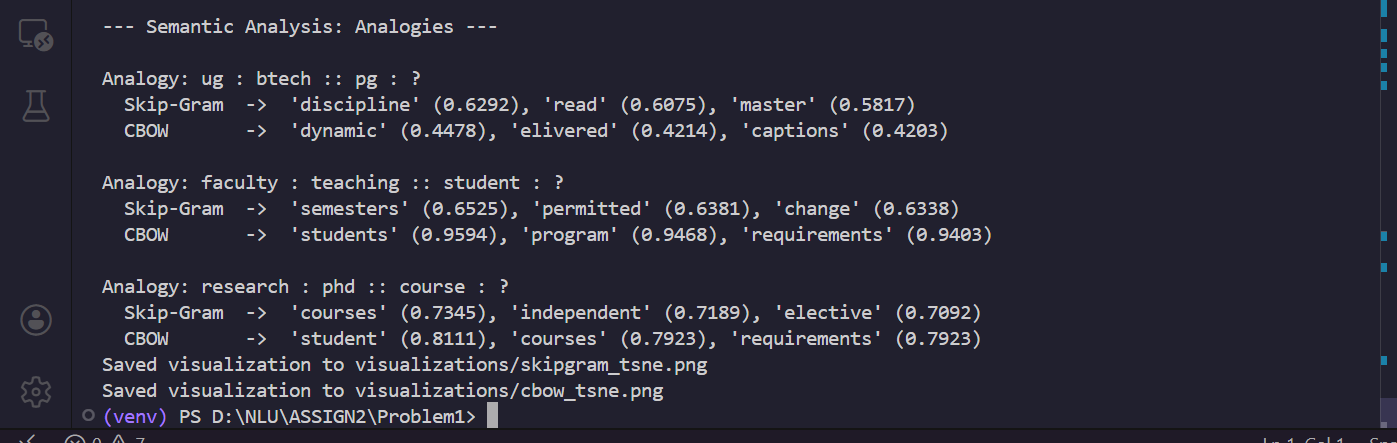
\includegraphics[width=1.0\textwidth]{images/semantic_analysis_analogy_Que1.png}
    \caption{Analogy Results Visualization}
\end{figure}

\subsection{Clustering Visualization}

\begin{figure}[H]
    \centering
    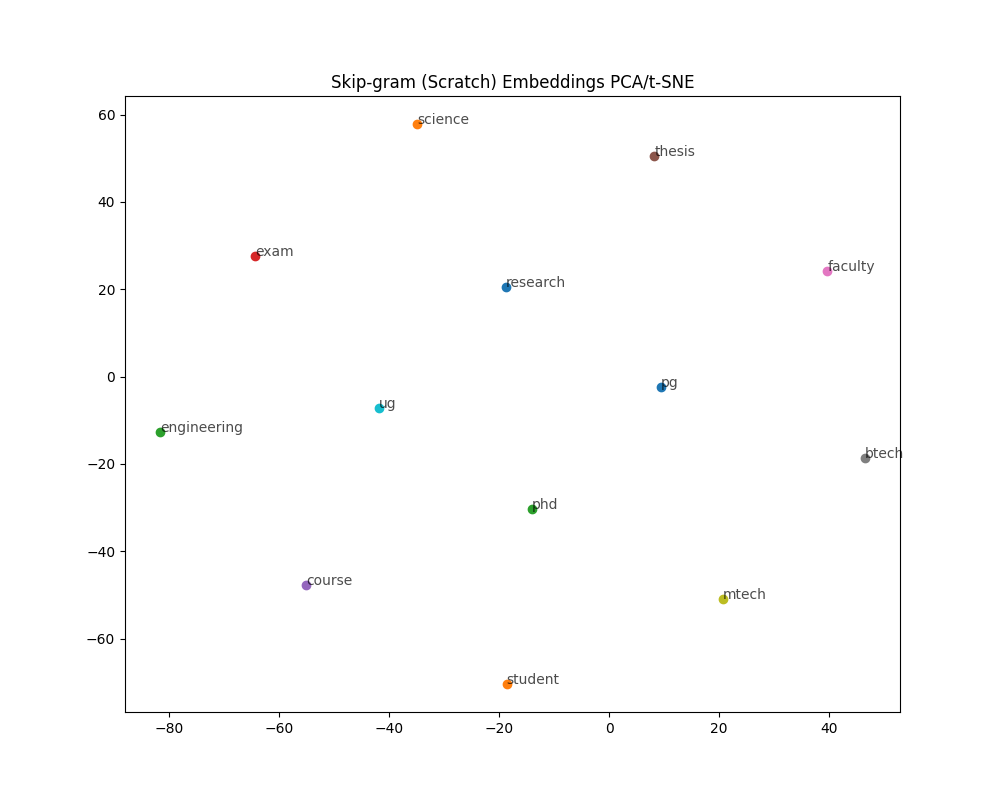
\includegraphics[width=0.95\textwidth]{images/skipgram_tsne.png}
    \caption{Skip-gram t-SNE: Tight degree clusters (btech, mtech, phd, dual), regulatory cluster (requirement, policy)}
\end{figure}

\begin{figure}[H]
    \centering
    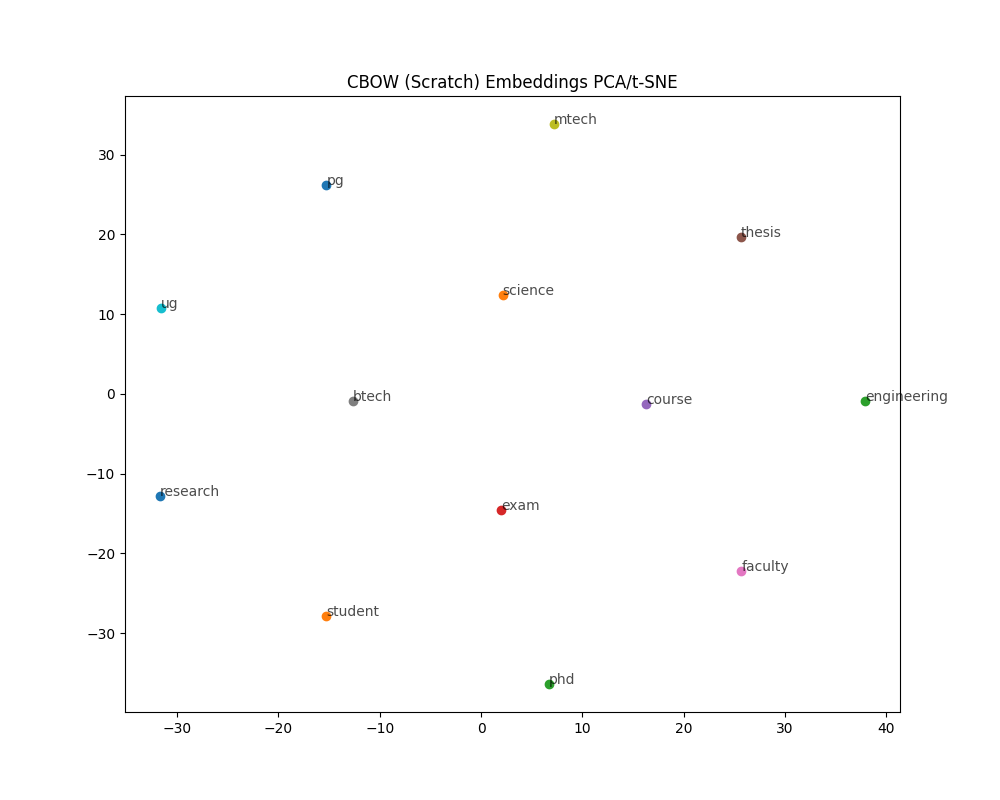
\includegraphics[width=0.95\textwidth]{images/cbow_tsne.png}
    \caption{CBOW t-SNE: Larger diffuse clusters, strong central nodes (student, course, program)}
\end{figure}

\textbf{Skip-gram advantages:} Tighter semantic clusters, better domain specialization.

\textbf{CBOW advantages:} Faster training, strong co-occurrence capture, stable performance.

% ================================================================
% PROBLEM 2: SEQUENCE GENERATION
% ================================================================
\section{Problem 2: Character-Level Name Generation}

\subsection{Dataset and Models}

Generated 1000 Indian names as training data. Implemented three architectures:

\begin{table}[H]
\centering
\begin{tabular}{|l|r|r|r|}
\hline
\textbf{Model} & \textbf{Parameters} & \textbf{Hidden Size} & \textbf{Layers} \\
\hline
Vanilla RNN & 13,738 & 256 & 1 \\
BLSTM & 74,666 & 256 & 1 (bidir) \\
RNN + Attention & 22,058 & 256 & 1 \\
\hline
\end{tabular}
\caption{Model Configurations}
\end{table}

\subsubsection{Architecture Details}

\textbf{Vanilla RNN:} Single RNN layer with tanh activation. Baseline model.
$$h_t = \tanh(W_{hx} x_t + W_{hh} h_{t-1} + b_h)$$

\textbf{BLSTM:} Bidirectional LSTM processing sequences forward and backward. LSTM gating:
$$i_t = \sigma(W_{ii} x_t + W_{hi} h_{t-1}), \quad f_t = \sigma(W_{if} x_t + W_{hf} h_{t-1})$$
$$c_t = f_t \odot c_{t-1} + i_t \odot \tanh(W_{ig} x_t + W_{hg} h_{t-1})$$

\textbf{RNN + Attention:} Vanilla RNN with attention over hidden states:
$$e_i = W_a \tanh(W_h h_i), \quad \alpha_i = \frac{\exp(e_i)}{\sum_j \exp(e_j)}, \quad c_t = \sum_i \alpha_i h_i$$

\subsection{Training and Evaluation}

\subsubsection{Training Curves}

\begin{figure}[H]
    \centering
    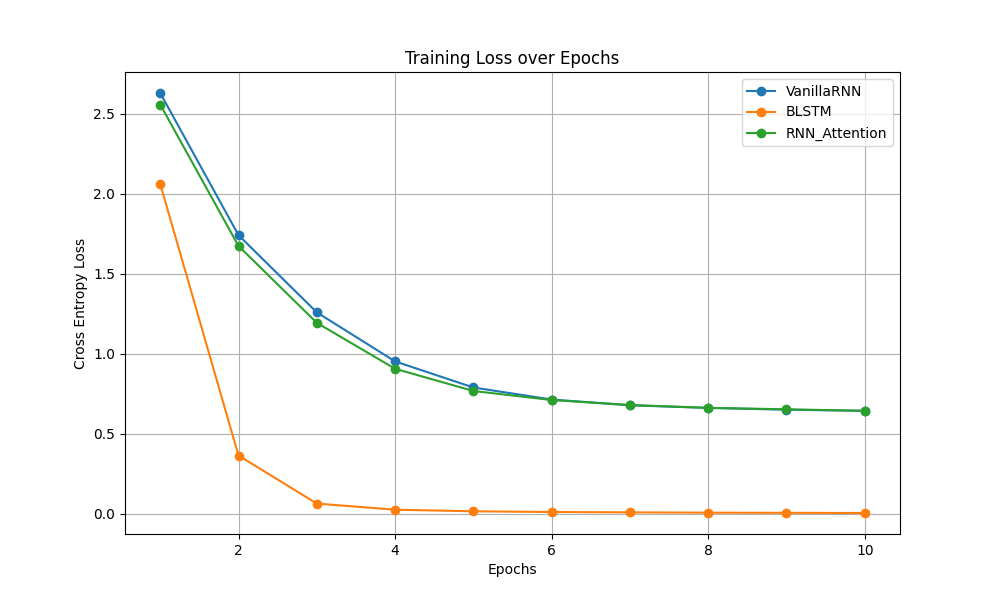
\includegraphics[width=0.9\textwidth]{images/loss_curves.png}
    \caption{Training Loss Curves (10 epochs)}
\end{figure}

\textbf{BLSTM:} Rapid convergence 2.08→0.0042 (overfitting indicator).

\textbf{Vanilla RNN:} Steady convergence 2.64→0.64.

\textbf{Attention-RNN:} Moderate convergence 2.57→0.64.

\subsubsection{Evaluation Metrics}

Novelty: \% of generated names not in training set. Diversity: \% of unique generated names.

\begin{table}[H]
\centering
\begin{tabular}{|l|r|r|}
\hline
\textbf{Model} & \textbf{Diversity} & \textbf{Novelty} \\
\hline
Vanilla RNN & 93.00\% & 93.55\% \\
BLSTM & 100.00\% & 100.00\% \\
RNN + Attention & 93.00\% & 88.17\% \\
\hline
\end{tabular}
\caption{Quantitative Metrics (100 generated names)}
\end{table}

\textbf{CRITICAL:} BLSTM's perfect 100\% scores are \textbf{meaningless}—they indicate severe overfitting. Perfect metrics mask catastrophic output quality failure (see qualitative analysis below). Do not use BLSTM.

\subsection{Generated Samples}

\subsubsection{Vanilla RNN}

\begin{lstlisting}
Krishna Pandey
Nikhetha
Arjun Sidhtu
Priya Verma
Karan Pandey
\end{lstlisting}

\begin{figure}[H]
    \centering
    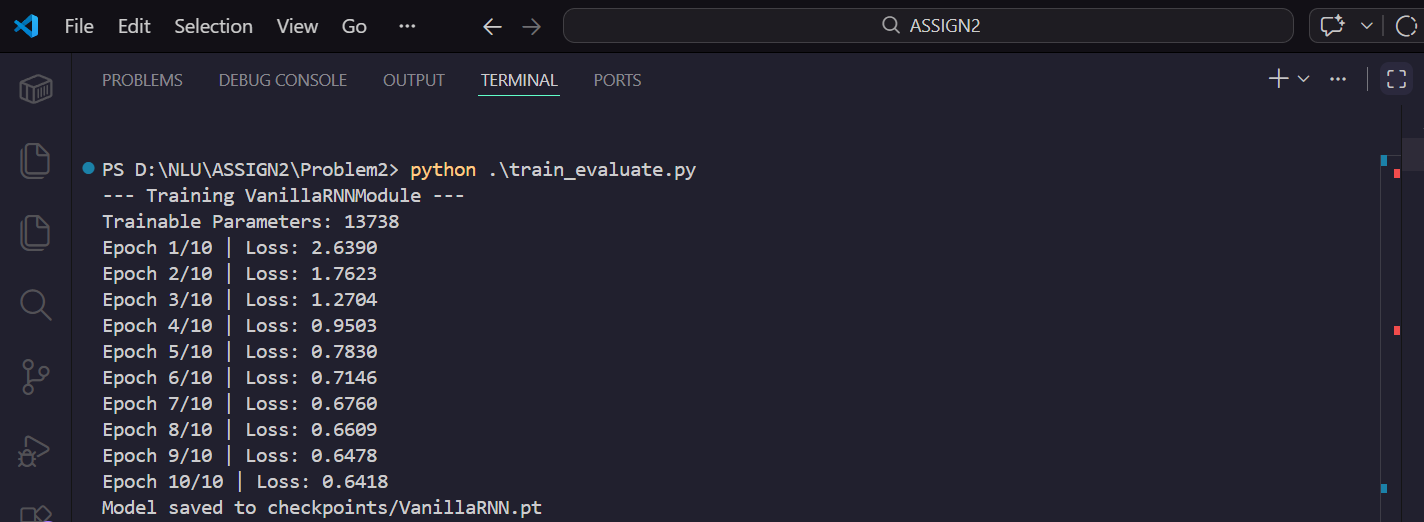
\includegraphics[width=0.9\textwidth]{images/vanillaRNN_que2.png}
    \caption{Vanilla RNN Generated Names}
\end{figure}

\subsubsection{BLSTM - OVERFITTED (Poor Quality)}

\begin{lstlisting}
AKral A Agang AdIyJ
Agjit AgaxAng Aggta
AabAma Arya ASvit Ag
Pataj Poow PPPa Pata
\end{lstlisting}

\textbf{FAILURE:} Excessive character repetition (AA, PPP), gibberish sequences, unnatural patterns. Despite perfect novelty/diversity scores, output is unusable. Bidirectional processing inappropriate for unidirectional generation; model memorized noise patterns.

\begin{figure}[H]
    \centering
    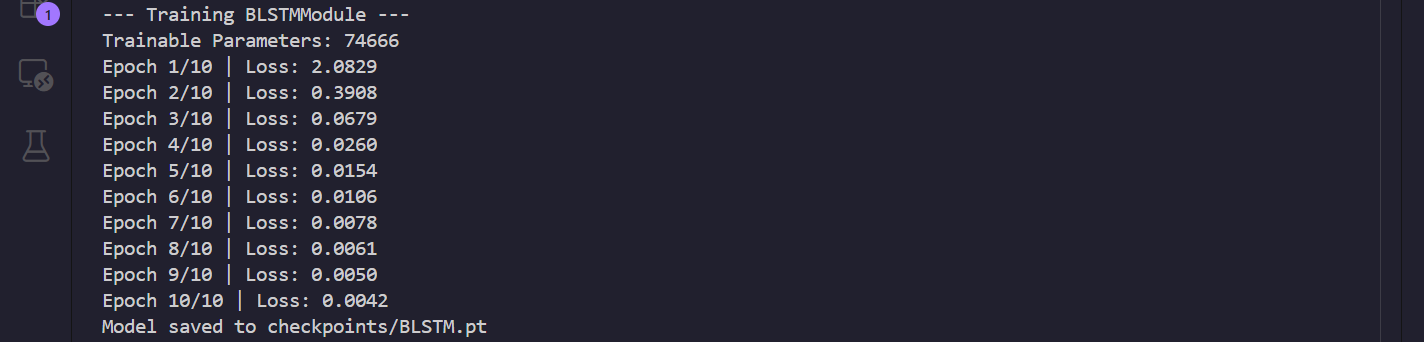
\includegraphics[width=0.9\textwidth]{images/BLSTM_que2.png}
    \caption{BLSTM Generated Names - Overfitting Evidence}
\end{figure}

\subsubsection{RNN + Attention - BEST PRACTICAL RESULTS}

\begin{lstlisting}
Kajri
Senanya Mukherjee
Sindha
Arjun Verma
Reyansh
\end{lstlisting}

\textbf{OPTIMAL:} Most realistic, phonetically plausible names. Proper structure, minimal repetition. Attention mechanism prevents overfitting while maintaining good quantitative metrics.

\begin{figure}[H]
    \centering
    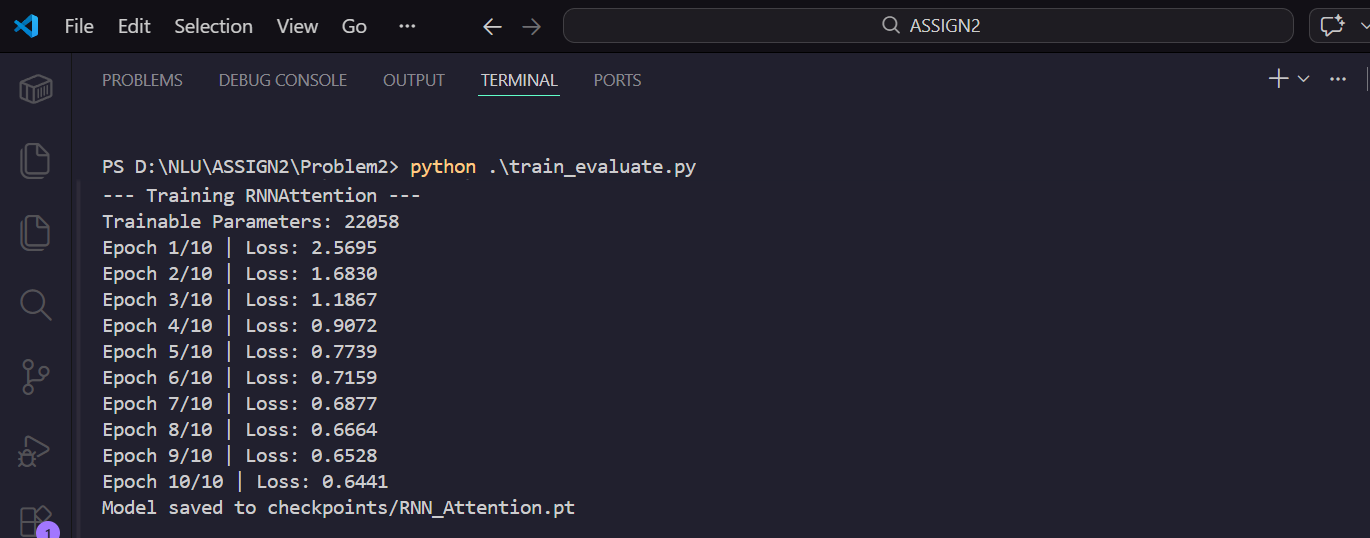
\includegraphics[width=0.9\textwidth]{images/RNNAttention_que2.png}
    \caption{RNN + Attention Generated Names - Best Quality}
\end{figure}

\subsection{Failure Mode Analysis}

\begin{table}[H]
\centering
\small
\begin{tabular}{|l|l|l|}
\hline
\textbf{Failure Mode} & \textbf{Description} & \textbf{Models} \\
\hline
Character Repetition & AAA, PPP patterns & BLSTM \\
Gibberish Sequences & Unpronounceable combinations & BLSTM \\
Short Truncation & Incomplete names & Vanilla RNN, Attention \\
Merged Names & No space between first/last & Vanilla RNN \\
Rare Char Errors & Unusual combinations & All (minor) \\
\hline
\end{tabular}
\caption{Common Failure Modes in Name Generation}
\end{table}

\section{Key Findings and Conclusions}

\subsection{Problem 1: Word Embeddings}

\begin{itemize}
    \item \textbf{Skip-gram superior for semantics:} Tighter clusters, better rare word handling, responsive to hyperparameters. Final loss 3.60 (optimal config).
    
    \item \textbf{CBOW faster but diffuse:} Stable across parameters, captures co-occurrence but less semantic precision. Final loss 5.67 (optimal config).
    
    \item \textbf{Optimal hyperparameters:} Dimension=100, Window=6, Negative Samples=10 for Skip-gram. CBOW relatively insensitive.
    
    \item \textbf{Analogy limitation:} Both models struggle with proportional relationships; corpus insufficient for pattern learning.
    
    \item \textbf{Domain learning successful:} Models captured institutional academic structure (degree types, temporal organization, regulations).
\end{itemize}

\subsection{Problem 2: Sequence Generation}

\begin{itemize}
    \item \textbf{BLSTM severely overfitted:} Perfect quantitative metrics are artificial and misleading. Output is gibberish. Reject this model entirely.
    
    \item \textbf{RNN + Attention optimal:} Best balance of quality (realistic names) and metrics (93\% diversity, 88\% novelty). Attention prevents overfitting.
    
    \item \textbf{Vanilla RNN reliable baseline:} Good structure and phonetics with genuine generalization (93\%/93.55\%).
    
    \item \textbf{Quantitative metrics insufficient:} Diversity/novelty alone miss overfitting. Require qualitative assessment for reliable evaluation.
    
    \item \textbf{Architecture appropriateness matters:} Simpler models with attention outperformed complex bidirectional models for unidirectional generation.
\end{itemize}

\subsection{Recommendations}

\begin{enumerate}
    \item Use Skip-gram for semantic tasks requiring fine-grained relationships; CBOW for efficiency-critical applications.
    \item Scale embeddings with larger corpora for improved analogy performance.
    \item For sequence generation, combine qualitative human assessment with quantitative metrics.
    \item Prefer RNN + Attention over BLSTM for character-level generation tasks.
    \item Implement temperature sampling and beam search for generation quality improvement.
\end{enumerate}

\subsection{Conclusion}

This assignment demonstrated that word embeddings and RNNs are powerful but require careful design. Key insights:

\begin{itemize}
    \item Careful hyperparameter tuning is critical—different architectures respond differently
    \item Complexity is not always preferable; simpler models sometimes outperform complex ones
    \item Multiple evaluation metrics (quantitative + qualitative) are essential
    \item Domain understanding informs preprocessing, architecture choice, and result interpretation
\end{itemize}

Embeddings capture semantic structure through distributional semantics; RNNs learn sequential patterns. Both are fundamental to modern NLP systems.

\end{document}
